% ============================================================
% 03-proposed-model.tex — CTU-Chat Proposed Architecture
% ============================================================
\section{Proposed Model}
\label{sec:model}

This section presents the architecture, algorithms, and evidence-acquisition mechanisms of \system{}. The proposed model is organized around three design principles: \emph{centralized agent coordination}, in which a contract-checked supervisor dispatches each query to one domain agent without peer-to-peer delegation; \emph{heterogeneous knowledge allocation}, which assigns each information structure to a corresponding evidence representation; and \emph{representation-aware evidence routing}, which selects either a direct graph-tool path or an intent-scoped retrieval path according to the assigned domain. Each \emph{specialist} is configured with domain-specific prompts, a scoped evidence path, and a restricted tool registry.

%------------------------------------------------
\subsection{Overall Proposed Architecture}
\label{sec:architecture}

Figure~\ref{fig:architecture} illustrates the system architecture of \system{}, structured across three coordinated tiers: (1)~the \emph{Interaction and Centralized Supervisor Tier}, (2)~the \emph{Domain-Specialized Multi-Agent Core Layer}, and (3)~the \emph{Heterogeneous Knowledge Storage and Tool Tier}.

\begin{figure}[t]
\centering
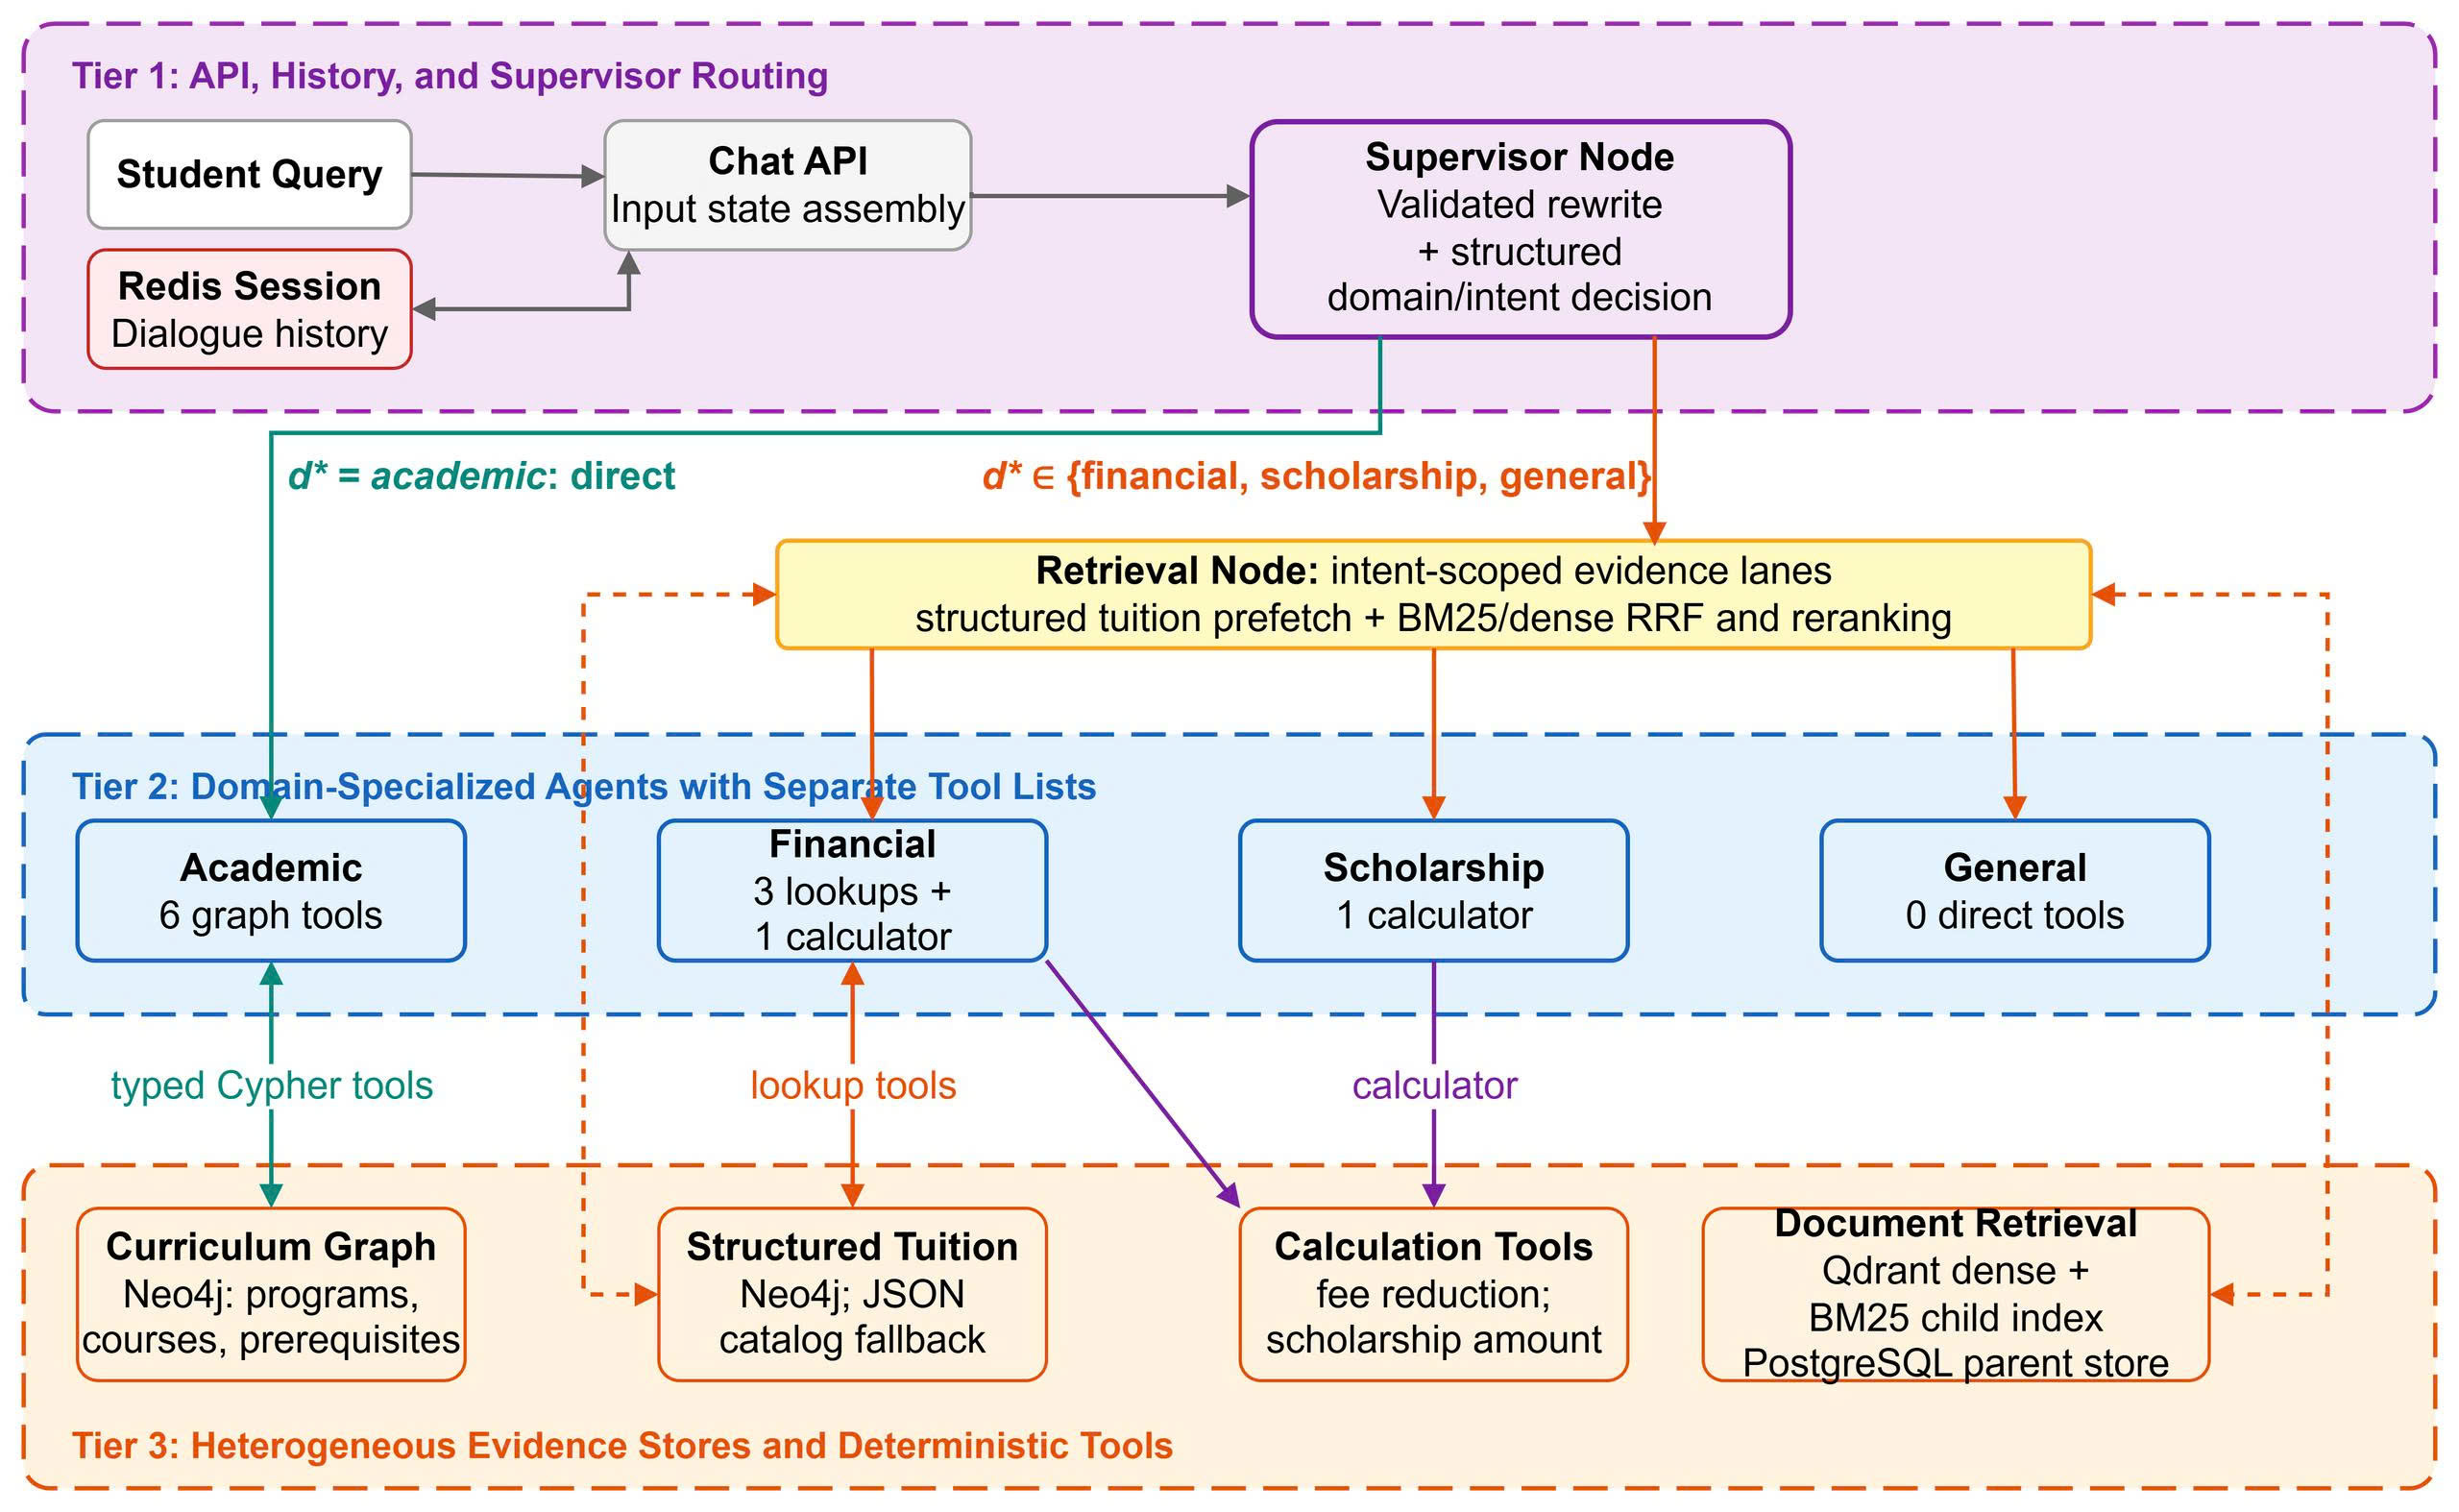
\includegraphics[width=\textwidth]{figures/architecture.jpg}
\Description{Diagram of the three-tier CTU-Chat system architecture. The top tier shows the interaction layer with a centralized supervisor router. The middle tier contains four domain-specialized agents: an academic graph agent connected to Neo4j, a financial agent with deterministic arithmetic tools, a scholarship agent with hybrid retrieval, and a general administrative agent. The bottom tier shows the heterogeneous knowledge storage layer comprising Neo4j graph database, PostgreSQL parent-chunk store, Qdrant vector index, and Redis session history. Solid arrows denote direct tool access and dashed arrows denote retrieval-node evidence acquisition. A contract-repair mechanism validates and may correct the supervisor's routing decision before conditional dispatch.}
\caption{Implemented \system{} architecture. Redis history enters the graph state; the supervisor's structured decision is contract-checked and may be repaired before conditional dispatch (repair is internal, not a separate node). Academic queries enter the graph-enabled agent, whereas other domains pass through intent-scoped retrieval. Solid and dashed links denote direct tool access and retrieval-node evidence acquisition, respectively.}
\label{fig:architecture}
\end{figure}


\textbf{Application-Level Specialization of LangGraph StateGraph:}
\system{} specializes LangGraph through typed state, an intent--owner contract, isolated paths, and partitioned tool registries. The contract checks structured supervisor output before dispatch; specialists then operate without peer delegation and see only their assigned tools.
\begin{itemize}
    \setlength{\itemsep}{1.5pt}
    \setlength{\parsep}{0pt}
    \setlength{\parskip}{0pt}
    \item \textbf{Node-scoped state:} \texttt{AgentState} retains the validated rewrite, raw and repaired routes, repair reason, evidence, and response; each node writes only its corresponding fields.
    
    \item \textbf{Conditional routing:} Deterministic edges send academic queries directly to the graph agent and all other queries through retrieval before dispatch to the selected financial, scholarship, or general agent.
    
    \item \textbf{Acyclic orchestration:} Specialists have no peer edges and return to \texttt{END}; their internal ReAct tool interactions are separate from the outer graph.
    
    \item \textbf{Asymmetric tools:} Academic, financial, and scholarship agents receive scoped lists, while the general agent has none. One bounded retry names an omitted required tool; invalid or missing parameters trigger clarification.
\end{itemize}

%------------------------------------------------
\subsection{Neo4j Knowledge Graph Specification and Cypher Tool Mechanics}
\label{sec:neo4j_graph}

\textbf{Schema defined by the ingestion layer:}
The Neo4j graph contains over 1,500 nodes and 3,800 edges across 113 undergraduate curricula and fee schedules. Its 10 node labels cover curriculum entities (e.g., \texttt{Program}, \texttt{Course}, and \texttt{Block}) and tuition entities (\texttt{TuitionFee}, \texttt{TuitionPolicy}, and \texttt{ExemptionBasisRate}); 13 typed relationships encode containment, prerequisites, program outcomes, tracks, occupations, tuition, and exemption bases. Narrative regulations remain in the document store.

\textbf{Cypher tool mechanics:}
The system does not ask the LLM to generate arbitrary Cypher. After the supervisor selects the academic agent, its ReAct policy chooses one of six typed tools and supplies the tool arguments. The tool normalizes identifiers or names and calls a fixed, parameterized Cypher query in the graph service. The tools implement three query classes:
\begin{itemize}
    \setlength{\itemsep}{1.5pt}
    \setlength{\parsep}{0pt}
    \setlength{\parskip}{0pt}
    \item \emph{Attribute lookup and search}: \texttt{tra\_cuu\_nganh} and \texttt{tim\_nganh} match program codes or normalized program, unit, and course names; \texttt{so\_sanh\_nganh} applies the same lookup before comparing two programs.
    \item \emph{Structural traversal}: \texttt{xem\_chuoi\_tien\_quyet} follows \texttt{REQUIRES} paths up to ten hops and returns direct \texttt{PARALLEL\_WITH} courses. \texttt{mon\_chung\_giua\_nganh} computes a course intersection across two program--block paths, and \texttt{tim\_nganh\_co\_mon} traverses those paths in reverse.
    \item \emph{Structured financial lookup}: parameterized queries match \texttt{TuitionFee}, \texttt{TuitionPolicy}, and \texttt{ExemptionBasisRate} properties and their program relationships. This graph lookup is separate from the BM25--dense hybrid document retrieval path used for narrative regulations.
\end{itemize}
This design binds agent actions directly to deterministic graph operations: the LLM only selects the appropriate tool and supplies its arguments, while the query topology remains fixed and parameterized within the graph service. The multi-agent workflow therefore incorporates graph evidence through bounded operations, reducing exposure to the syntactic and semantic errors associated with unconstrained Cypher generation.

%------------------------------------------------
\subsection{Algorithmic Foundations: Routing and Deterministic Arithmetic}
\label{sec:algorithms}

For a query $q$ and its most recent dialogue predecessor, the supervisor first attempts a validated standalone rewrite. It then predicts domain $d_{\mathrm{raw}}$ and intent $\iota_{\mathrm{raw}}$ under a structured schema, falling back to \texttt{general}/\texttt{other} on parsing failure. The ownership contract repairs strong rule conflicts or incompatible domain--intent pairs and records both raw and repaired decisions in the shared state. Academic queries proceed directly to the graph agent; other domains build intent-scoped retrieval lanes, with financial queries first attempting Neo4j tuition lookup and then JSON fallback. The selected specialist receives the resulting state and terminates at \texttt{END}.

\textbf{Deterministic Tuition Reduction Arithmetic:}
For fee-reduction requests, \system{} augments the LLM with the external deterministic tool \texttt{tinh\_toan\_hoc\_phi}. The LLM interprets the request and supplies three parameters---the actual per-credit tuition $T$, the per-credit exemption basis $B$, and the percentage entitlement $p$---but does not perform the arithmetic through free-form text generation. The external tool validates the percentage range and applies the fixed calculation
\begin{equation}
  D = B\frac{p}{100}, \qquad P = \max(0, T-D).
  \label{eq:tuition_reduction}
\end{equation}
where $D$ is the reduction per credit and $P$ is the remaining amount per credit. Monetary inputs are expected in VND per credit. The tool enforces $0 \le p \le 100$ and clamps $P$ at zero; values outside the percentage range return an error.

Rather than a new general-purpose algorithm, the contribution lies in composing validated rewriting, constrained routing, representation-specific dispatch, and deterministic arithmetic within the multi-agent workflow.

%------------------------------------------------
\subsection{Heterogeneous Knowledge Allocation and Hybrid Retrieval}
\label{sec:hybrid_retrieval}

This layer implements \emph{heterogeneous knowledge allocation}: rather than forcing all institutional knowledge into a uniform document index, \system{} preserves relational curriculum knowledge in Neo4j, accesses cohort-dependent tuition data through structured lookup, and retains narrative regulations and scholarship policies in document retrieval.

The access policy maps program attributes to Neo4j property lookup, prerequisite and shared-course questions to graph traversal, regulation identifiers to BM25, paraphrased regulations to hybrid RRF with reranking, and fee or scholarship arithmetic to deterministic Python tools.

At runtime, academic queries enter the graph agent directly; other domains enter retrieval. Financial retrieval first attempts Neo4j tuition lookup with JSON fallback. The repaired intent then selects metadata-filtered document lanes, and packed evidence is passed only to the selected specialist.

\textbf{Hybrid Document Retrieval Path.}
For narrative regulations and scholarship criteria, BM25 and Qdrant search 400-character child chunks; their parent sections are loaded from PostgreSQL and fused using $s_{\mathrm{RRF}}(d)=\sum_{s\in\{\mathrm{bm25},\mathrm{dense}\}}(60+r_s(d))^{-1}$. The full configuration pools intent-governed candidates with the top 20 unfiltered hybrid candidates and top BM25 anchors, deduplicates them, and reranks with \texttt{BAAI/bge-reranker-v2-m3}. Scores below 0.20 are removed unless fewer than two candidates remain; graph evidence is then added under fixed quotas and up to seven passages are packed for generation.

Parent sections use a 2,800-character target with 100-character overlap;
child chunks use a 400-character target with 50-character overlap.
